\documentclass[a4paper, 12pt]{article}
\usepackage[total={17cm,25cm}, top=2.5cm, left=2.5cm, right=2.5cm,  includefoot]{geometry}
\usepackage[utf8]{inputenc}
\usepackage{array}
\usepackage{multirow}
\usepackage{hhline}
\usepackage{gensymb}
\usepackage{graphicx}
\graphicspath{ {} }
\usepackage[czech]{babel}
\usepackage{enumitem}
\usepackage{pdfpages}
\usepackage{amsmath}
\usepackage{verbatim}
\usepackage{listings}
\usepackage{hyperref}
\usepackage{amssymb}


\pagestyle{empty} % vypne číslování stránek




\usepackage[OT2,OT1]{fontenc}
\newcommand\cyr
{
\renewcommand\rmdefault{wncyr}
\renewcommand\sfdefault{wncyss}
\renewcommand\encodingdefault{OT2}
\normalfont
\selectfont
}
\DeclareTextFontCommand{\textcyr}{\cyr}
\def\cprime{\char"7E }
\def\cdprime{\char"7F }
\def\eoborotnoye{\char’013}
\def\Eoborotnoye{\char’003}


\begin{document}



\begin{titlepage}
\begin{center}
\noindent
\Large \textbf{České vysoké učení technické v Praze }\\ Fakulta stavební
\vspace{5cm}

\huge

%vložení loga cvut
\begin{figure}[h!]
	\centering
	
\includegraphics[width=7cm]{logo.png}
\end{figure}

\vspace{0.5cm}

Algoritmy v digitální kartografii \\

\vspace{3cm}

\Huge  
Digitální model terénu a jeho analýzy\\

\vspace{2cm}

\Large
Bc. Robin Pflug \\
Bc. Tomáš Klemsa \\

\end{center}

\end{titlepage}




\pagestyle{plain}     % zapne obyčejné číslování
\setcounter{page}{1}  % nastaví čítač stránek znovu od jedné

\tableofcontents
\newpage

\section{Zadání úlohy}

\textbf{Vstup:} \textit{množina} $P=(p_1,...,p_n),p_i=[x_i,y_i,z_i]$.\\
\textbf{Výstup:} 	\textit{polyedrický DMT nad množinou P představovaný vrstevnicemi doplněný vizualizací sklonu trojúhelníků a jejich expozicí.}\\

Metodou inkrementální konstrukce vytvořte nad množinou P vstupních bodů 2D Delaunay triangulaci. Jako vstupní data použijte existující geodetická data (alespoň 300 bodů) popř. navrhněte algoritmus pro generování syntetických vstupních dat představujících významné terénní tvary (kupa, údolí, spočinek, hřbet, ...).\\
\\
Vstupní množiny bodů včetně níže uvedených výstupů vhodně vizualizujte . Grafické rozhraní realizujte s využitím frameworku QT. Dynamické datové struktury implementujte s využitím STL. \\
\\
Nad takto vzniklou triangulací vygenerujte polyedrický digitální model terénu. Dále proveĎte tyto analýzy:
\\
\begin{itemize}
  \item S využitím lineární interpolace vygenerujte vrstevnice se zadaným krokem a v zadaném intervalu, proveďte jejich vizualizaci s rozlišením zvýrazněných vrstavnic.
  \item Analyzujte sklon DMT, jednotlivé trojúhelníky vizualizujte v závislosti na jejich sklonu.
  \item Analyzujte expozici digitálního modelu terénu, jednotlivé trojúhelníky vizualizujte v závislosti na jejich expozici ke světové straně. 
\end{itemize}

Zhodnoťte výsledný DMT z kartografického hlediska, zamyslete se nad slabinami algoritmu založeného na 2D Delaunay triangulaci. Ve kterých situacích nebude dávat vhodné výsledky? Tyto situace graficky znázorněte. \\

\subsection{Bonusové úlohy}

Ze zadání bonusových úloh byla řešena \textit{Barevná hypsometrie} a \textit{Výběr barevných stupnic při vizualizaci sklonu a expozice}.  
\begin{figure}[h!]
	\centering
	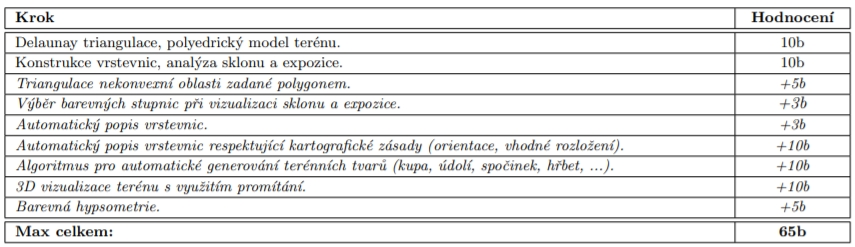
\includegraphics[width=15cm]{hodnoceni.jpg}
	\caption{Bodové hodnocení úlohy [zdroj: 1]}
\end{figure}

\newpage
\section{Obecná formulace a řešení problému}
\textbf{Delaunayho triangulace:} Při triangulaci množiny bodů, je žádoucí aby vytvořené trojúhelníky byly co nejvíce rovnostranné. Pokud to takto provedeme, každý trojúhelník by měl co nejlépe lokálně reprezentovat hodnotu povrchu. Další požadovaná charakteristika triangulačního procesu je, aby byla produkována jednoznačná triangulace nezávisle na počátečním bodě nebo orientaci množiny dat. Tyto výsledky budou předpověditelné a jednoduše opakovatelné. Sibson (1978) ukázal, že Dalaunayho triangulace tyto podmínky obecně splňuje, i přes to, že jsou určité konfigurace množiny dat (jako např. pravoúhlý GRID) která má na výstupu lokálně nejednoznačné řešení. [zdroj: 3]\\
\\
\textbf{Digitální model terénu:} Digitální model terénu (DMT) je digitální popis a prezentace reálného povrchu jako 2D nebo 3D model, který se skládá z reálných naměřených dat a interpolačních metod, které dopočítávají pravděpodobná data pro místa, kde data chybí. Uvnitř modelovaného území je možno v libovolných bodech odvodit nadmořské výšky. [zdroj: 2]\\
\\
\textbf{Barevná hypsometrie:} Barevná hypsometrie je kartografická technika znázornění terénního reliéfu na mapě, a to pomocí vrstevnic a plošného vybarvení jednotlivých výškových vrstev mezi nimi, tedy znázornění nadmořské výšky v mapách metodou vyplnění barevných ploch. [zdroj: 2]\\
\\

\begin{figure}[h!]
	\centering
	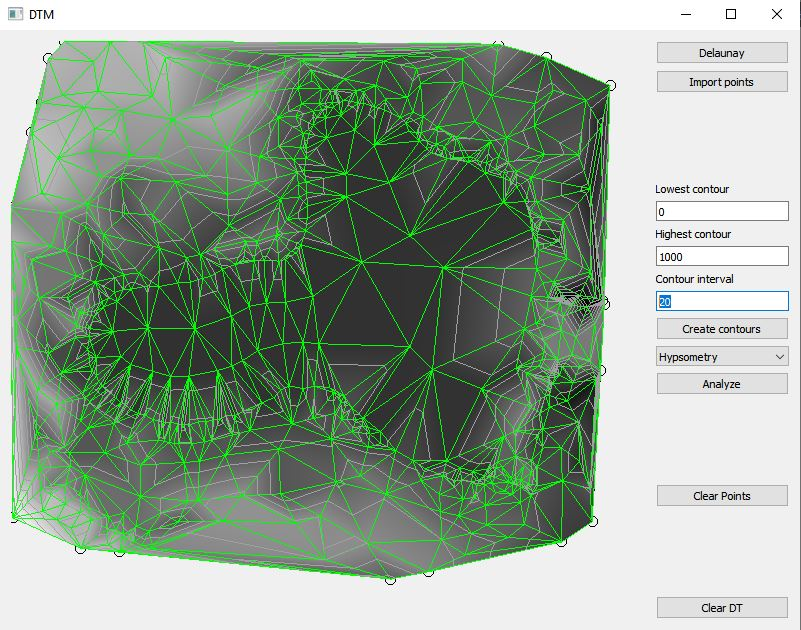
\includegraphics[width=10cm]{test25.jpg}
	\caption{Barevná hypsometrie}
\end{figure}

Zadáním této úlohy bylo vytvořit aplikaci, které nad zadanou množinou bodů vytvoří metodou inkrementální konstrukce 2D Delaunay triangulace. Takto vzniklá triangulace bude generovat digitální model terénu. V aplikaci dále budou dvě metody pro analýzu DTM: \textit{sklon} a \textit{expozici}. Nad DTM bude možné se zadaným krokem vygenerovat vrstavnice. Jako bonusová část úlohy je metoda, která vytvoří nad DTM barevnou hypsometrii.

\section{Aplikované algoritmy}
Algoritmy využívané pro tvorbu triangulace nad množinou bodů, digitálního modelu terénu, generaci vrstevnic a barevné hypsometrie.

\subsection{Delaunay triangulace}
Pro tvorbu triangulace byla použita Delaunay. Tato triangulace je nejběžnější pro metody tvořící digitální model terénu.\\
\\
Algoritmus, který byl použit tvoří triangulaci \textit{inkrementální konstrukcí}: Hrany mají danou orientaci a postupně jsou hledané takové body, které náleží levé polorovině dané hranou a zároveň s body hrany tvoří minimální opsanou kružnici.  Existuje-li takovýto bod, pak generuje dvě nové hrany, které jsou přidány do triangulace. Nepodaří-li se bod splňující tato kritéria nalézt, pak se orientace hrany otočí a bod je opět hledán. \\
\\
Jednotlivé hrany jsou ukládány do listu aktivních hran (\textit{AEL}). Pokud k hraně v \textit{AEL} bude nalezen třetí bod, podle výše uvedených kritérií, bude hrana z listu vyjmuta. V \textit{AEL} je také kontrolováno, zda se vkládaná hrana v listu již nenachází ovšem s opačnou orientací. Celý algoritmus probíha, dokud list aktivních hran není prázdný. 

\begin{figure}[h!]
	\centering
	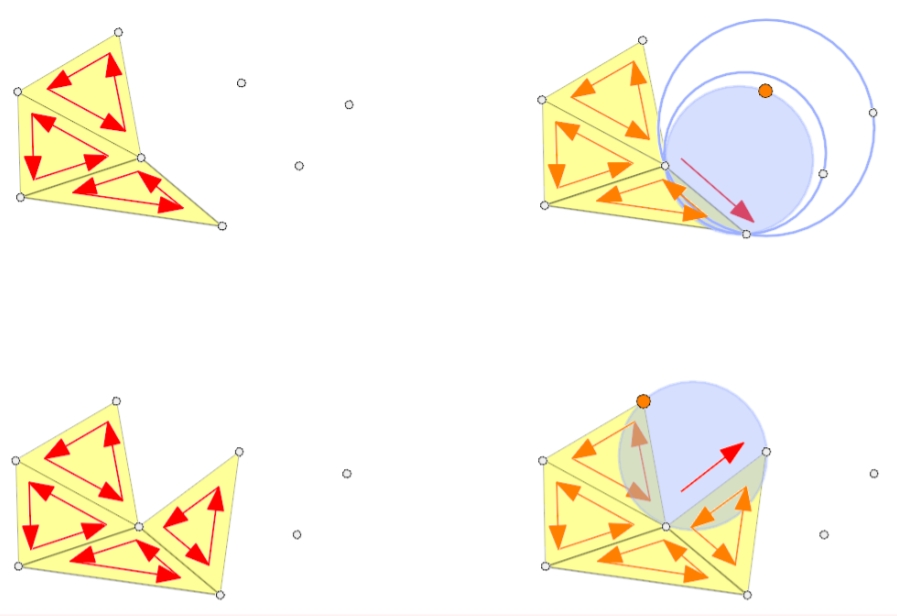
\includegraphics[width=12cm]{inkrementalni_triangulace.jpg}
	\caption{Inkrementální konstukce DT [zdroj: 1]}
\end{figure}

\subsubsection{Algoritmus DT Incremental}
\begin{enumerate}
\item Nalezení pivota $p_1 = rand(P), ||p_2 - p_1|| = min$
\item Vytvoř hranu e $e = (p_1, p_2 $//Nalezení prvních dvou bodů tvořících hranu. 
\item $p_{-} =arg min_{\forall p_i\epsilon \sigma_{l}(e)} r'(k_i), k_i = (a,b,p_i), e = (a,b)$/
\item Pokud $\nexists p_{-}$, prohoď orientaci $e \leftarrow (p_2,p_1)$. Jdi na \textit{3.}.
\item $e_2 = (p_2, p_{-}), e_3 = (p_{-}, p_1)$ //Zbívající hrany trojúhelníku§
\item $AEL \leftarrow e, AEL \leftarrow e_2, AEL \leftarrow e_3$//Přidání hran do listu aktivních hran
\item $\textit{DT} \leftarrow e, \textit{DT} \leftarrow e_2, \textit{DT} \leftarrow e_3$//Přidání hran do \textit{DT}
\item while AEL not empty:
\subitem $AEL \rightarrow e, e = (p_1,p_2)$ // Vezmi první hranu z AEL
\subitem $e = (p_2, p_1)$// Prohoď jejich orientaci
\subitem $p_{-} =arg min_{\forall p_i\epsilon \sigma_{l}(e)} r'(k_i), k_i = (a,b,p_i), e = (a,b)$
\subitem if $\exists p_{-}:$ //Bod existuje
\subsubitem $e_2 = (p_2, p_{-}), e_3 = (p_{-},p_1)$ //Zbyvajici hrany trojúhelníku
\subsubitem $\textit{DT} \leftarrow e$ // Přidej hratu do \textit{DT} ale ne do AEL
\subsubitem $add(e_2, AEL, \textit{DT}), add(e_3, AEL, \textit{DT})$ // Přidej do \textit{DT} i do AEL
\end{enumerate}

\subsubsection{Algoritmus DT Incremental - add}
\begin{enumerate}
\item Vytvoř hranu $e' = (b,a)$
\item if $(e' \epsilon AEL)$
\subitem $AEL \rightarrow e'$
\item else:
\subitem $AEL \leftarrow e$
\item \textit{DT} $\leftarrow (a,b)$
\end{enumerate}[zdroj: 1]

\newpage
\subsection{Vrstevnice}
Vsrtevnice je křivka, která v modelu spojuje body o stejné nadmořské výšce. Vrstevnice jsou generovány v pravidelném intervalu.

\begin{figure}[h!]
	\centering
	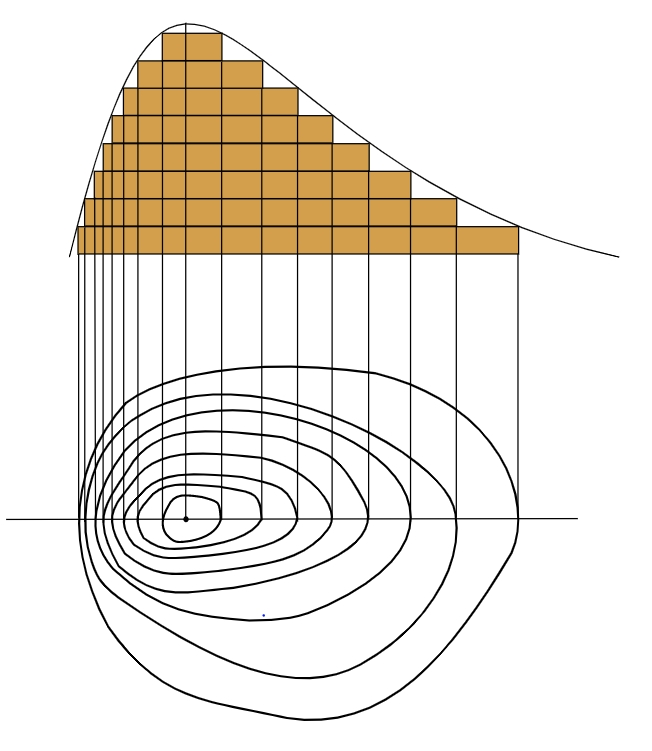
\includegraphics[width=9cm]{vrstevnice.jpg}
	\caption{Grafické znázornění tvorby vrstevnic [zdroj: 2]}
\end{figure}

Vrstevnice byly v této úloze tvořeny lineární interpolací. Jako vrstevnice byla vygenerována přímka průsečíku vodorovné roviny o dané nadmořské výšce a příslušného trojúhelníku z modelu. Rozestup vrstevnic mezi dvěma body byl volen jako konstantní. 

\subsubsection{Algoritmus tvorby vrstavnic}
\begin{enumerate}
\item Pro všechny hrany trojúhelníku t: $ \forall e_i \in t: $
\item Hrana náleží rovině vrstevnice z: $ (z - z_i) \cdot (z - z_{i+1}) = 0 \rightarrow e_i \in \rho $
\item Hrana nenáleží rovině vrstevnice z: $ (z - z_i) \cdot (z - z_{i+1}) < 0 \rightarrow e_i \not \in \rho $
\item Hrana je průnikem roviny vrstevnice z: $ (z - z_i) \cdot (z - z_{i+1}) < 0 \rightarrow e_i \cap \rho $
\subitem Výpočet polohových souřadnic: 
$$  x = \frac{(x_2 - x_1)}{(z_2 - z_1)} (z - z_1) + x_1 $$ 
$$  y = \frac{(y_2 - y_1)}{(z_2 - z_1)} (z - z_1) + y_1 $$ 
\subitem Vytvoř hranu tvořící vrstevnici.
\end{enumerate}

\newpage

\subsection{Sklon terénu}
Sklon terénu je určen jako úhel, který svírá normála roviny analyzovaného trojúhelníku a normála vodorovné roviny o velikosti 1. Sklon terénu byl graficky znázorněn stupněm odstínu šedé jednotlivých trojúhelníků. Tmavší odstín v analýze sklonu je důsledkem většího sklonu plošky. 

\begin{figure}[h!]
	\centering
	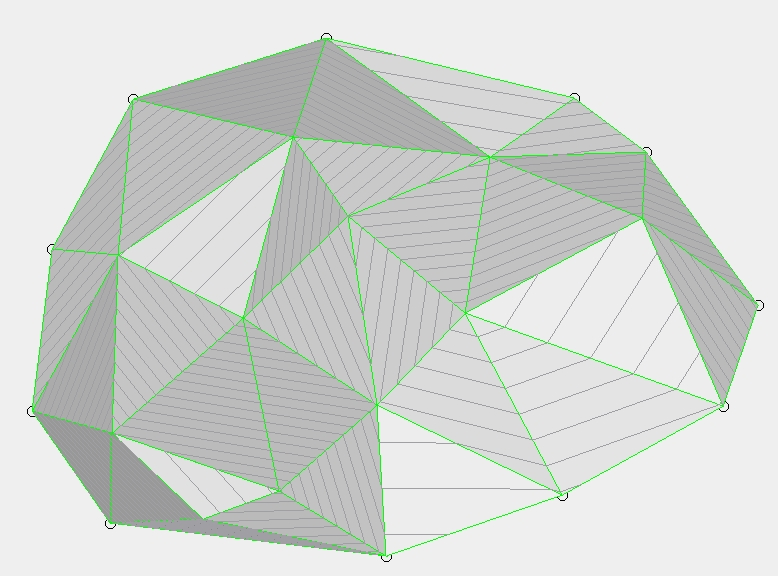
\includegraphics[width=14cm]{sklon.jpg}
	\caption{Grafické znázornění sklonu}
\end{figure}

\subsubsection{Algoritmus analýzy sklonu}
\begin{enumerate}
\item Pro všechny trojúhelníky triangulace: $ \forall t_i \in DT: $
\subitem Výpočet normálového vektoru roviny trojúhelníku: \\
 $$ n_t = (u_y \cdot v_z - u_z \cdot v_y)^2 - (u_x \cdot v_z - u_z \cdot v_x)^2  + (u_x \cdot v_y - u_y \cdot v_x)^2 $$
\subitem Kde:
$$  u_x = \Delta x_2, x_1; u_y = \Delta y_2, y_1; u_z = \Delta z_2, z_1;$$
$$  v_x = \Delta x_2, x_3; u_y = \Delta y_2, y_3; u_z = \Delta z_2, z_3;$$
\item Výpočet sklonu: $ \varphi = arccos \frac{n_z}{|n_t|} $
\end{enumerate}
\newpage

\subsection{Expozice terénu}
Analýza expozice terénu je počítána jako azimut průmětu normálového vektoru trojúhelníku do rovny tvořené osami \textit{x} a \textit{y}. Expozice znázorňuje orientaci trojúhelníku tvořící model, vůči světovým stranám.\\
\\
Pro vizualizaci expozice byl použit kulový barevný model \textit{HSV} převedený do RGB. Tento barevný model nejvíce odpovídá lidskému vnímání barev. Skládá se ze tří složek (nejsou to základní barvy), u nichž je nutno hlídat hodnoty (možné nesmyslné kombinace):
\begin{itemize}
\item Hue – odstín
\item Saturation – sytost barvy
\item Value – hodnota jasu
\end{itemize}

\begin{figure}[h!]
	\centering
	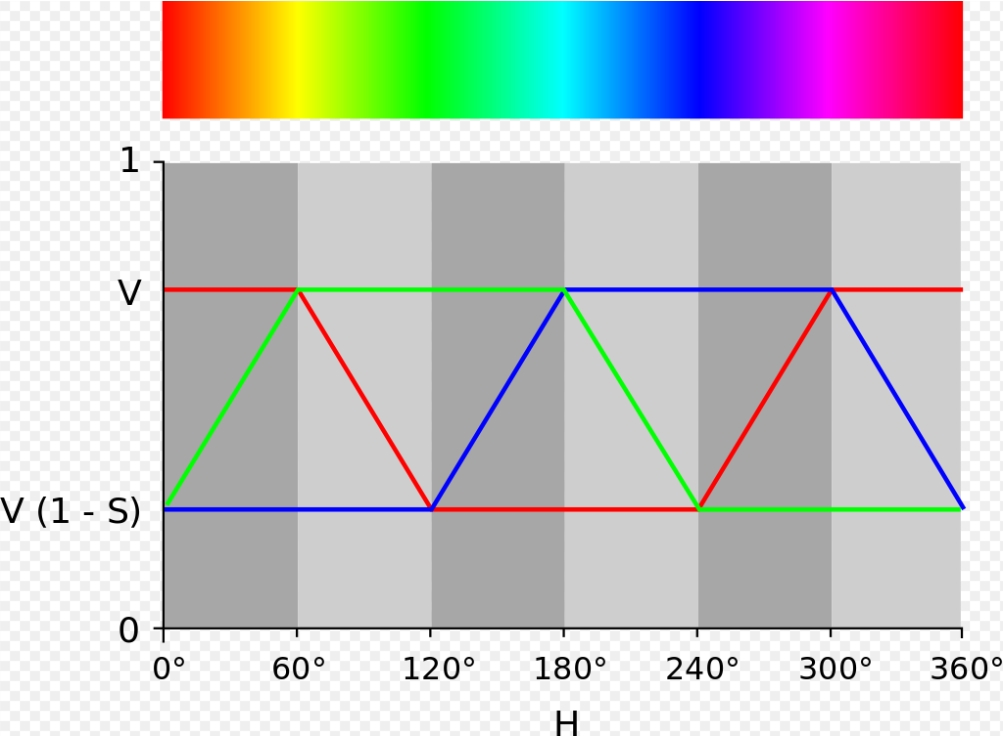
\includegraphics[width=11cm]{HSV.jpg}
	\caption{Převod HSV modelu do RGB [zdroj: 2]}
\end{figure}

\subsubsection{Algoritmus analýzy expozice}
\begin{enumerate}
\item Pro všechny trojúhelníky triangulace: $ \forall t_i \in DT: $
\subitem Výpočet x a y části normálového vektoru: \\
$$ n_x = (u_y \cdot v_z - u_z \cdot v_y) $$
$$ n_y = -(u_x \cdot v_z - u_z \cdot v_x) $$
\subitem Kde:
$$  u_x = \Delta x_2, x_1; u_y = \Delta y_2, y_1; u_z = \Delta z_2, z_1;$$
$$  v_x = \Delta x_2, x_3; u_y = \Delta y_2, y_3; u_z = \Delta z_2, z_3;$$
\item Výpočet expozice: $ A =atan2( \frac{n_x}{n_y}) $
\end{enumerate}

\newpage

\section{Bonusové úlohy}

\subsection{Výběr barevných stupnic při vizualizaci sklonu a expozice}
Řešení této úlohy je popsáno v kapitole Aplikované algoritmy - \textit{Sklon terénu} a \textit{Expozice terénu}.

\subsection{Barevná hypsometrie}

Barevná hypsometrie spočívá ve vytvoření výškových vrstev ohraničených vrstevnicemi na rozhraní typických intervalů získaných z hypsografické křivky, a jejich vybarvení.\\
\\
Barevný hypsomerie byla vytvořena na principu barevné škály "čím výše, tím světleji". Výhodou uvedeného postupu je stálost stupňování, které je přirozené pro kontinuitu povrchu terénu i přírodní výškové gradienty. [zdroj: 2]

\begin{figure}[h!]
	\centering
	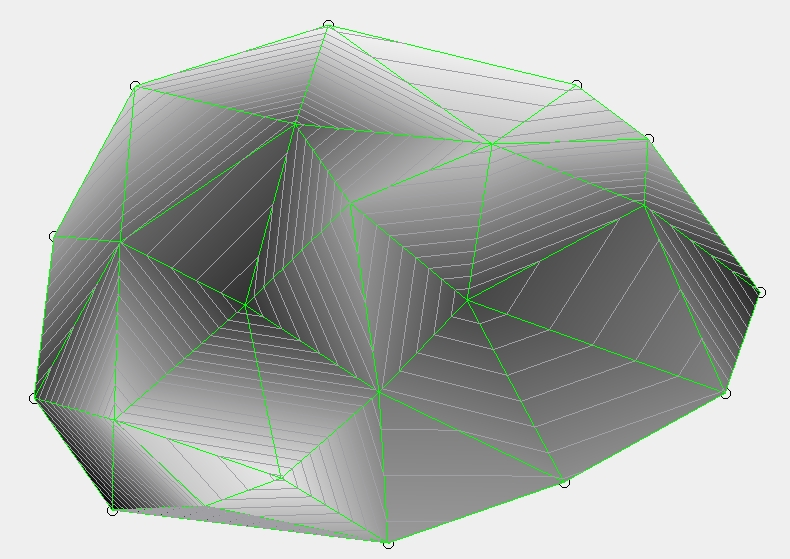
\includegraphics[width=12cm]{hypso.jpg}
	\caption{Barevná hypsometrie aplikovaná na DTM}
\end{figure}

\newpage

\section{Vstup dat do aplikace}
Vstup dat v aplikaci lze realizovat dvěma způsoby. Uživatel sám vkládá body do grafického okna za pomoci kurzoru myši nebo hromadně načte soubor ve formátu .txt obsahující strukturovaně uspořádané souřadnice bodů (viz vzor). Vkládaná množina bodů musí obsahovat zredukované souřadnice Z. Tato souřadnice musí být redukována na interval od 0 do 255. V případě, že hodnoty Z nepokrývají interval, je vhodné je přeškálovat na celý interval.\\
\\
Grafický vstup souřadnic, tvořený kurzorem je náhodný. Proto je vhodný spíše pro testování programu.\\
\\
 
\begin{figure}[h!]
	\centering
	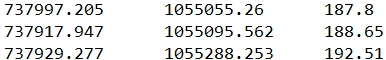
\includegraphics[width=8cm]{data.jpg}
	\caption{Vzor vstupních dat pro nahrávaní ze souboru .txt}
\end{figure}

\section{Výstup aplikace}
Grafický výstup je prezentován v Canvasu grafického rozhraní.

\begin{figure}[h!]
	\centering
	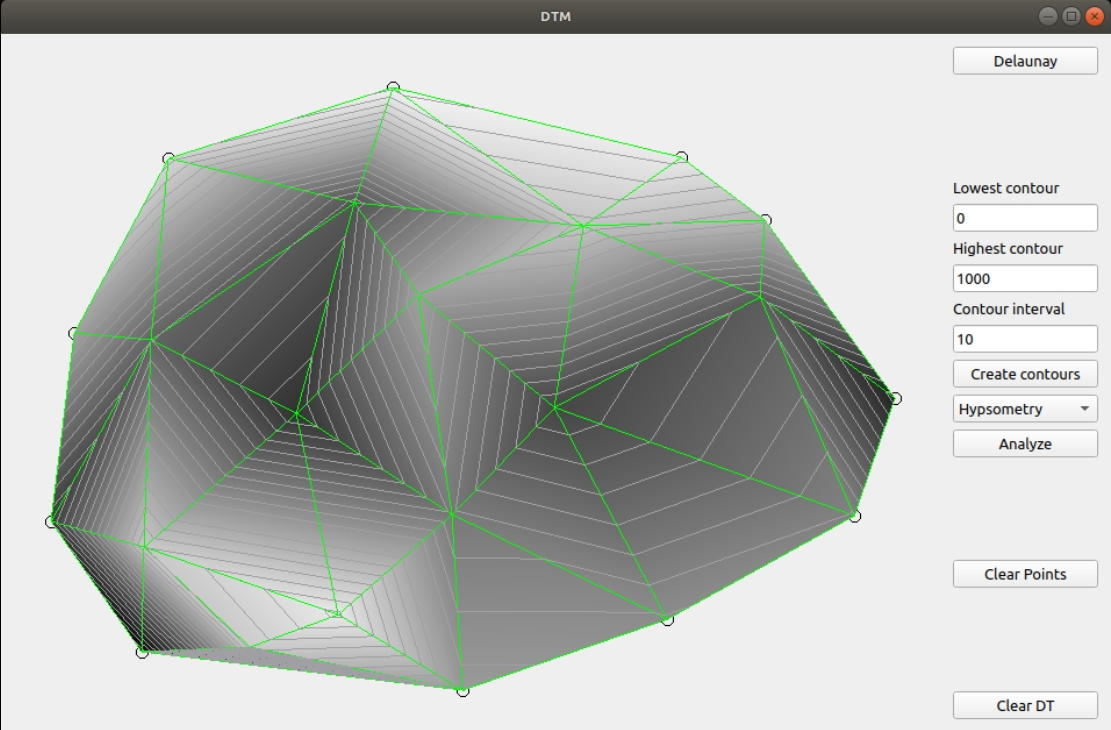
\includegraphics[width=12cm]{vystup.jpg}
	\caption{Grafické okno aplikace}
\end{figure}

\section{Dokumentace}
\subsection{Třídy}
\subsubsection{Algorithms}
Třída Algorithms obsahuje metody zajišťující výpočty daných algoritmů.
\\

\textbf{int getPointLinePosition(QPoint3D q,QPoint3D p1,QPoint3D p2)}\\
Návratová hodnota: \textit{integer};\\
Metoda vrátí polohu bodu \textit{q} vůči přímce dané body\textit{ p1} a \textit{p2}. Hodnota 1 je pro polohu vlevo od přímky, 0 pro polohu vpravo od přímky a -2 pro polohu bodu na přímce.
\\

\textbf{double getCircleRadius(QPoint3D p1, QPoint3D p2, QPoint3D p3, QPoint3D c)}\\
Návratová hodnota: \textit{double};\\
Metoda vrátí polomě kružnice dané třemi body.
\\

\textbf{int getNearestpoint(QPoint3D p, std::vector$<QPoint3D>$ points)}\\
Návratová hodnota: \textit{integer};\\
Metoda navrací index nejbližšího bodu vzhledem k bodu \textit{p} z vkládaného vektoru bodů \textit{points}. 
\\

\textbf{double distance2Points(QPoint3D p1, QPoint3D p2)}\\
Návratová hodnota: \textit{double};\\
Metoda vrátí velikost vzdálenosti dvou bodů.
\\

\textbf{int getDelaunayPoint(QPoint3D s, QPoint3D e, std::vector$<QPoint3D>$, points)}\\
Návratová hodnota: \textit{int};\\
Metoda navrátí index ideálního Delaunay bodu ze zadaného vektoru bodů, vůči zadané úsečce.  
\\


\textbf{std::vector$<Edge>$ DT(std::vector$<QPoint3D>$ points)}\\
Návratová hodnota: \textit{vector$<Edge>$};\\
Metoda navrací vektor hran tvořící Delaunayho triangulaci. 
\\

\textbf{QPoint3D getContourPoint(QPoint3D p1, QPoint3D p2, double z)}\\
Návratová hodnota: \textit{QPoint3D};\\
Metoda vrací bod vrstevnice. Bod byl určen jako průsečík zadané přímky a vodorovné roviny o zadané výšce.
\\

\textbf{vector$<Edge> createContourLines$(vector$<Edge> dt$, double $z_min$, double $z_max$, double dz)}\\
Návratová hodnota: \textit{vector$<Edge>$};\\
Metoda vytvoří a navrátí vektor obsahující hrany vrstevnice. 
\\

\textbf{double calculateSlope(QPoint3D p1, QPoint3D p2, QPoint3D p3)}\\
Návratová hodnota: \textit{double};\\
Metoda navrací hodnotu sklonu zadaného trojúhelníku. 
\\

\textbf{double calculateAspect(QPoint3D p1, QPoint3D p2, QPoint3D p3)}\\
Návratová hodnota: \textit{double};\\
Metoda navrací hodnotu azimutu zadaného trojúhelníku. 
\\

\textbf{std::vector$<Triangle>$ analyzeDTM(std::vector$<Edge>$ dt)}\\
Návratová hodnota: \textit{vector$<Triangle>$};\\
Metoda navrací vektor analyzovaných trojúhelníků (tři body trojúhelníku, sklon a azimut) pro zadanou Delaunayho triangulaci. 

\subsubsection{Edge}
Třída Edge definuje hranu. Hrana je dána jako počáteční bod \textit{s} a koncový bod \textit{e}.\\

\textbf{QPoint3D getStart()}\\
Návratová hodnota: \textit{QPoint3D};\\
Metoda vracející počáteční bod linie.
\\

\textbf{QPoint3D getEnd()}\\
Návratová hodnota: \textit{QPoint3D};\\
Metoda vracející koncový bod linie.
\\

\textbf{void setStart(QPoint3D s)}\\
Návratová hodnota: \textit{void};\\
Metoda nastaví počáteční bod linie.

\textbf{void setEnd(QPoint3D e)}\\
Návratová hodnota: \textit{void};\\
Metoda nastaví koncový bod linie.

\subsubsection{QPoint3D}
Třída QPoint3D definuje bod o třech souřadnicích (x; y; z).
\\

\textbf{double getZ()}\\
Návratová hodnota: \textit{double};\\
Metoda vracející hodnotu souřadnice \textit{z}.
\\

\textbf{void setZ(double z)}\\
Návratová hodnota: \textit{void};\\
Metoda nastaví pro bod \textit{QPoint3D} souřadnici \textit{z}.

\subsubsection{SortbyX}
Třída SortbyX slouží k porovnání souřadnic v ose x.\\

\textbf{bool operator()(QPoint \&p1, QPoint \&p2)}\\
Přetížený operátor () vrátí bod s větší souřadnicí x z dvojice bodů.

\subsubsection{Triangle}
Třída Triangle definuje trojúhelník. Obsahuje tři vrcholy trojúhelníku \textit{QPoint3D}, s vrcholy nese trojúhelník i hodnotu sklonu a azimutu. 

\textbf{QPoint3D getP1()}\\
Návratová hodnota: \textit{QPoint3D};\\
Metoda vracející vrchol trojúhelníku P1. 
\\

\textbf{QPoint3D getP2()}\\
Návratová hodnota: \textit{QPoint3D};\\
Metoda vracející vrchol trojúhelníku P2. 
\\

\textbf{QPoint3D getP3()}\\
Návratová hodnota: \textit{QPoint3D};\\
Metoda vracející vrchol trojúhelníku P3. 
\\

\textbf{double getSlope()}\\
Návratová hodnota: \textit{double};\\
Metoda vracející hodnotu sklonu trojúhelníku. 
\\

\textbf{double getAspect()}\\
Návratová hodnota: \textit{double};\\
Metoda vracející hodnotu azimutu trojúhelníku. 
\\

\textbf{$void setP1(QPoint3D p1_-)$}\\
Návratová hodnota: \textit{void};\\
Metoda nastaví trojúhelníku vrchol P1. 
\\

\textbf{$void setP2(QPoint3D p2_-)$}\\
Návratová hodnota: \textit{void};\\
Metoda nastaví trojúhelníku vrchol P2. 
\\

\textbf{$void setP3(QPoint3D p3_-)$}\\
Návratová hodnota: \textit{void};\\
Metoda nastaví trojúhelníku vrchol P3. 
\\

\textbf{$void setSlope(double slope_-)$}\\
Návratová hodnota: \textit{void};\\
Metoda nastaví trojúhelníku sklon. 
\\

\textbf{$void setAspect(double aspect_-)$}\\
Návratová hodnota: \textit{void};\\
Metoda nastaví trojúhelníku azimut. 
\\

\newpage

\section{Testování}
Testování probíhalo na reálných open-source datech poskytovaných na stránkách geoportálu Prahy: www.geoportalpraha.cz. Jediná úprava spočívala v redukci výškových souřadnic viz kapitola \textit{Vstup dat do aplikace}. Z geoportálu byl stažen Digitální model terénu ve formátu shapefile. V softwaru QGis byly nad Digitálním modelem terénu části Prahy vygenerovány body v souřadicích S-JTSK a BpV. Vygenerovány byly 3 různé množiny bodů o rozdílné poloze a počtu.

\newpage

\subsection{Test 1}
První množina použita pro testování dat obsahovala 389 bodů. V terénu se nacházely lesy, budovy, dopravní komunikace i pole. 

 \begin{figure}[h!]
	\centering
	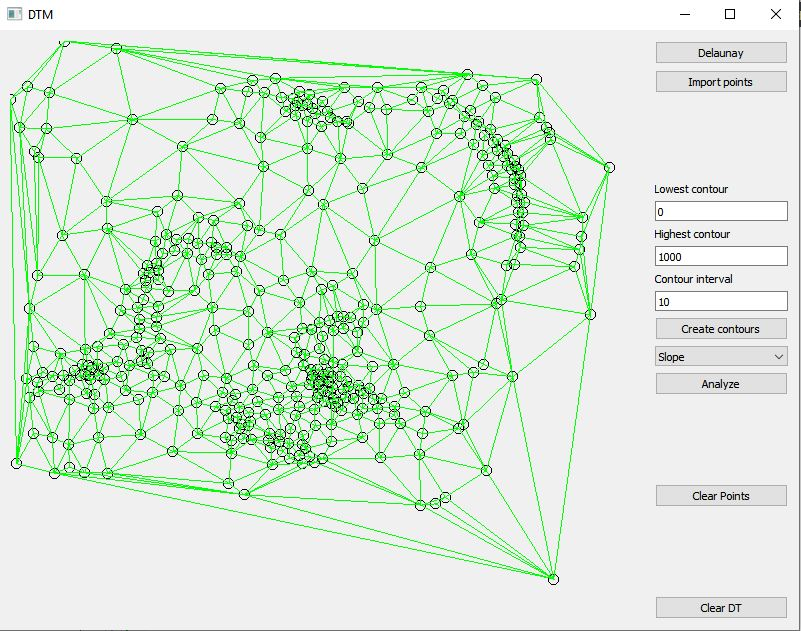
\includegraphics[width=10cm]{test11.jpg}
	\caption{Delaunay triangulace}
\end{figure}

 \begin{figure}[h!]
	\centering
	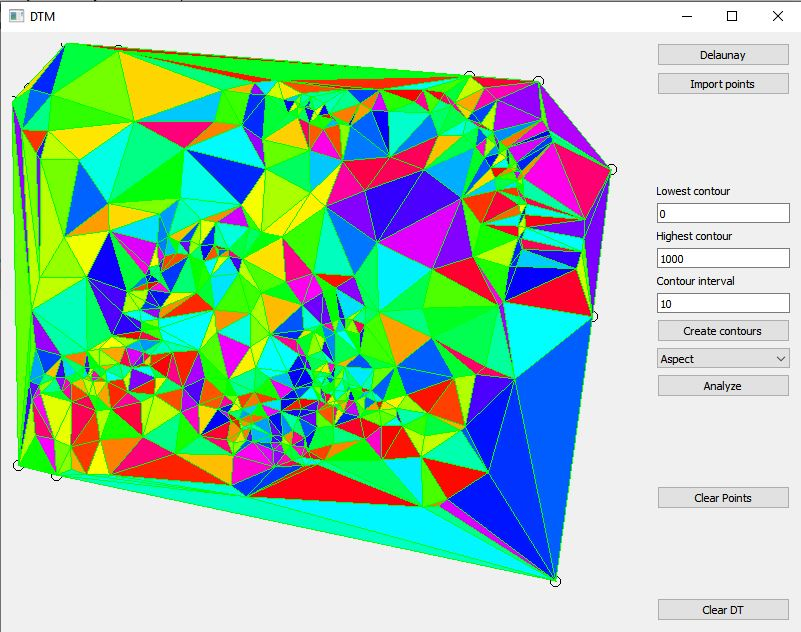
\includegraphics[width=10cm]{test12.jpg}
	\caption{Analýza azimutu}
\end{figure}

 \begin{figure}[h!]
	\centering
	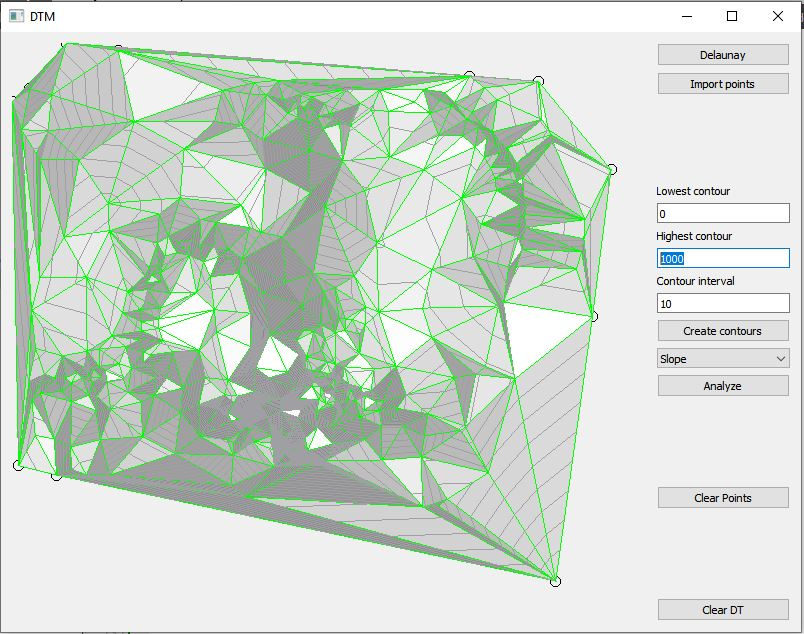
\includegraphics[width=10cm]{test14.jpg}
	\caption{Analýza sklonu}
\end{figure}

 \begin{figure}[h!]
	\centering
	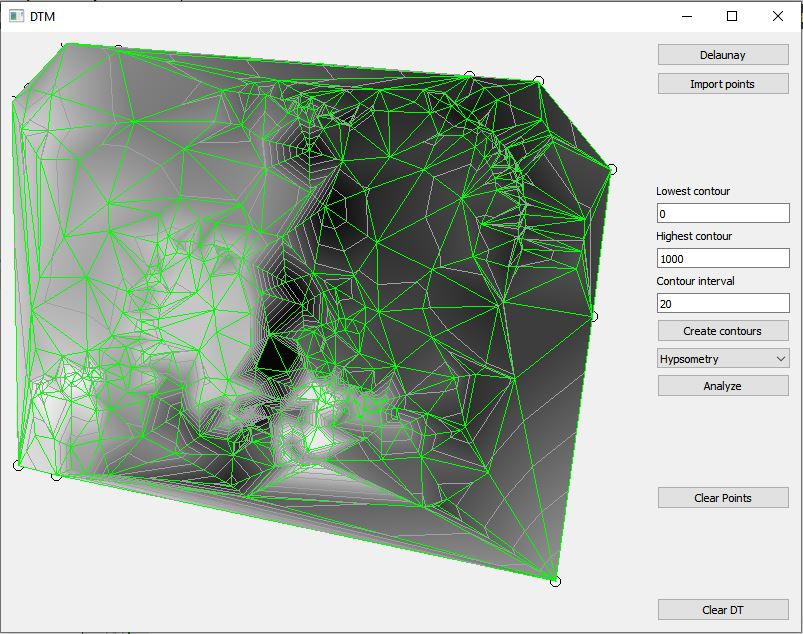
\includegraphics[width=10cm]{test15.jpg}
	\caption{Barevná hypsometrie}
\end{figure}

\clearpage

\subsection{Test2}
Druhá množina použita pro testování dat obsahovala 527 bodů. V terénu se nacházel rybník.

 \begin{figure}[h!]
	\centering
	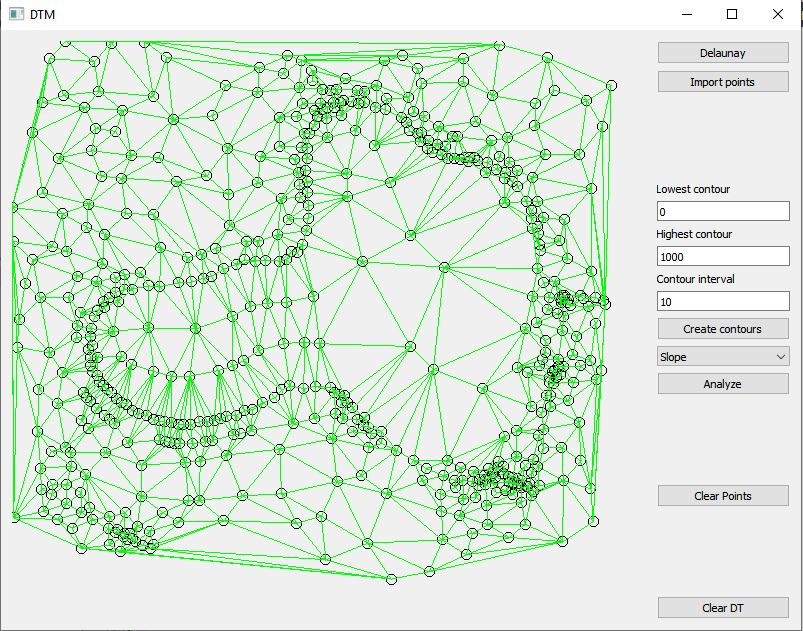
\includegraphics[width=10cm]{test21.jpg}
	\caption{Delaunay triangulace}
\end{figure}

 \begin{figure}[h!]
	\centering
	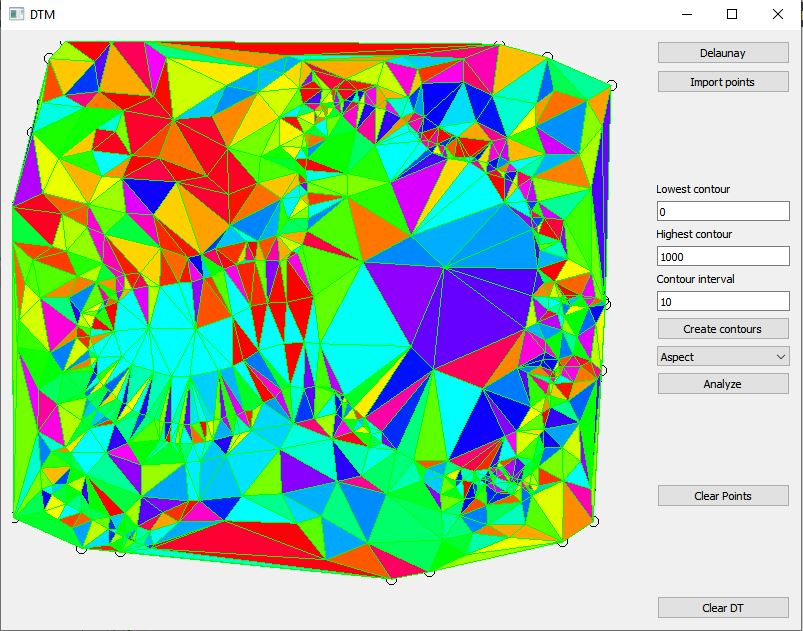
\includegraphics[width=10cm]{test22.jpg}
	\caption{Analýza azimutu}
\end{figure}

 \begin{figure}[h!]
	\centering
	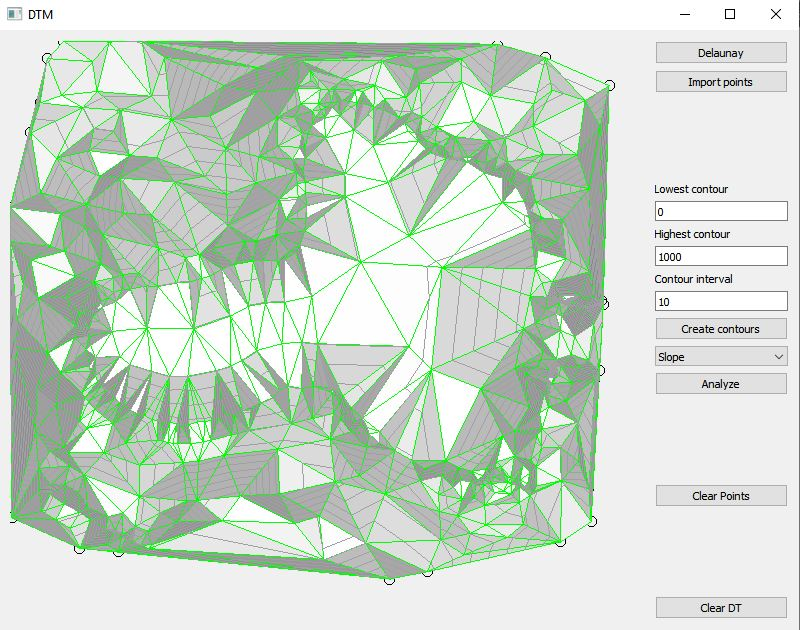
\includegraphics[width=10cm]{test24.jpg}
	\caption{Analýza sklonu}
\end{figure}

 \begin{figure}[h!]
	\centering
	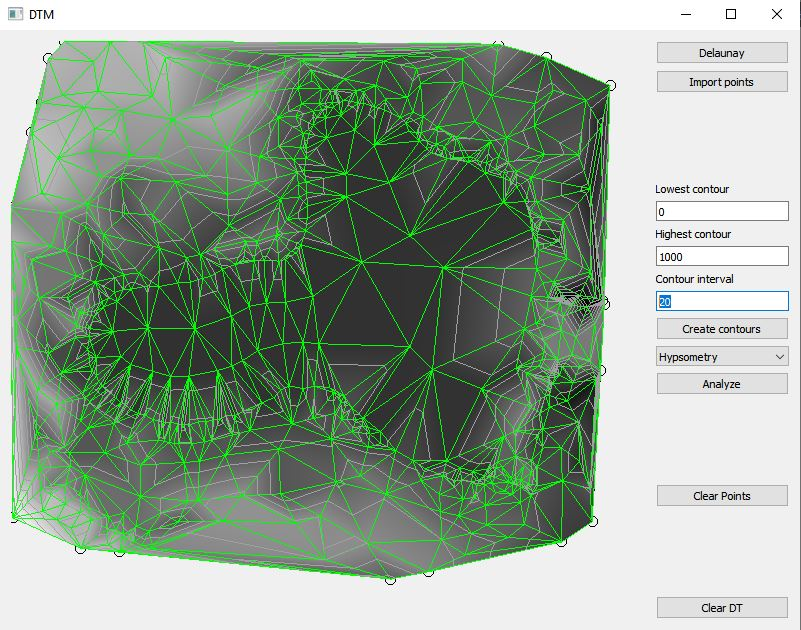
\includegraphics[width=10cm]{test25.jpg}
	\caption{Barevná hypsometrie}
\end{figure}

\clearpage

\subsection{Test3}
Třetí množina použita pro testování dat obsahovala 187 bodů. V terénu se nacházelo pole. Z aplikace lze pozorovat přesnot využitého modelu terénu. V důsledku přeškálování rozsahu souřadnice Z jsou zde vidět jednotlivé nerovnosti terénu. 

 \begin{figure}[h!]
	\centering
	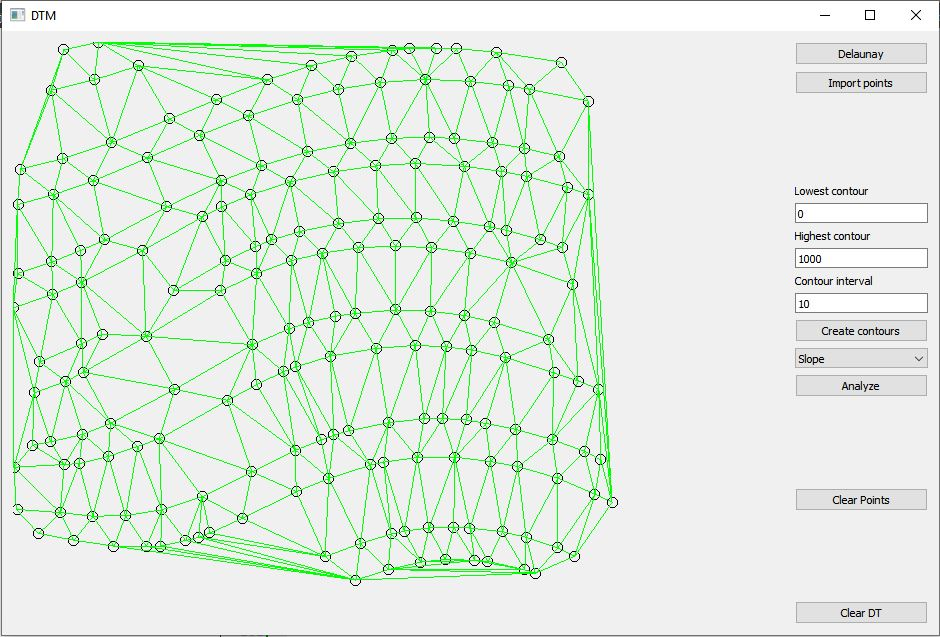
\includegraphics[width=10cm]{test31.jpg}
	\caption{Delaunay triangulace}
\end{figure}

 \begin{figure}[h!]
	\centering
	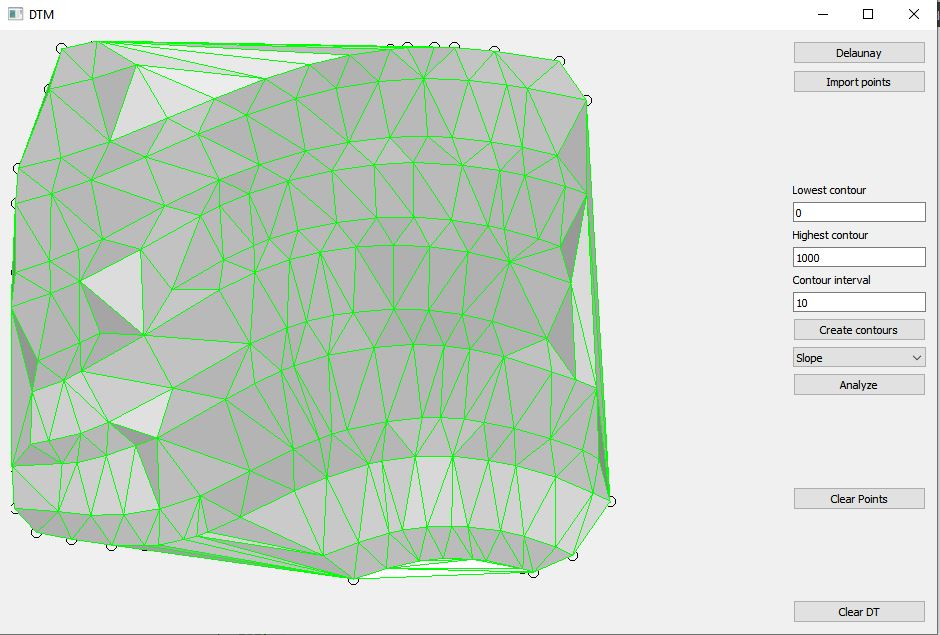
\includegraphics[width=10cm]{test32.jpg}
	\caption{Analýza azimutu}
\end{figure}

 \begin{figure}[h!]
	\centering
	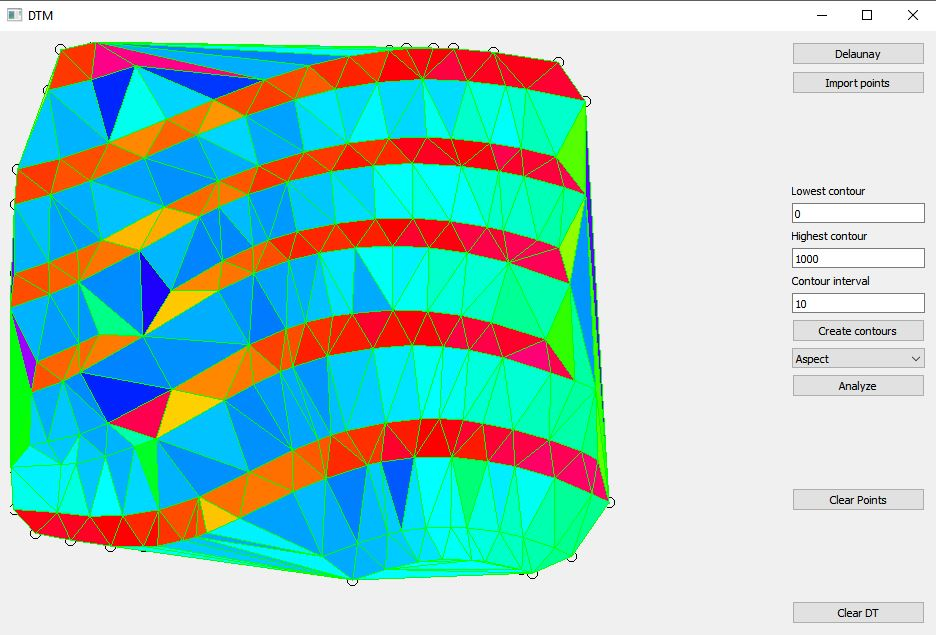
\includegraphics[width=10cm]{test33.jpg}
	\caption{Analýza sklonu}
\end{figure}

 \begin{figure}[h!]
	\centering
	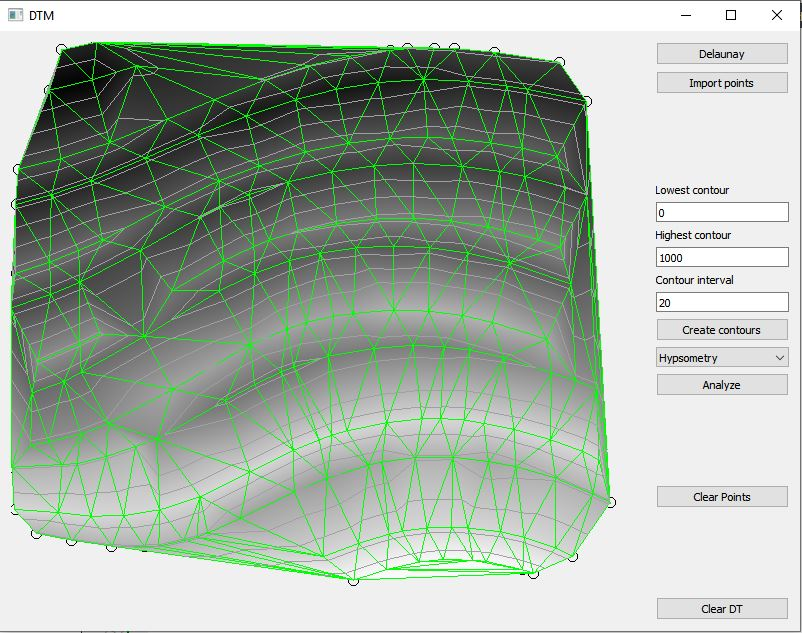
\includegraphics[width=10cm]{test35.jpg}
	\caption{Barevná hypsometrie}
\end{figure}

\clearpage

\section{Závěr}
Aplikace vytváří a analyzuje digitální model povrchu vytvořený Delaunay triangulací. Analyzován je sklon a azimut terénu (trojúhelníků). Aplikace dále vykresluje vrstevnice v zadaném intervalu a lze v ní generovat barevnou hypsometrii. \\
\\
Do aplikace lze nahravát i větší množiny bodů v tetovém formátu bez potřeby větších úprav. Proto lze aplikaci využít na modelaci a následnou analýzu naměřených hodnot rovinných území například metodou GNSS.

\section{Náměty pro vylepšení} 
Aplikace, konkrétně Delaunay triangulace, obecně selhává u bodů vytvářejících struktůru mřížky. Dále také selhává u určitých teréních tvarů (hrana, propast). Jako řešení těchto problémů se využívá povinných hran, které ovšem v aplikaci definovat nelze.\\
\\
Dalším zlepšení vyplývajícího ze předchozího odstavce je naopak vymazání existujících hran, které nedávají smysl.\\
\\
Pro vrstevnice by také bylo vhodnější generovat popis se skutečnými výškami v daném souřadnicovém systému. 

\section{Reference}

\begin{enumerate}

\item  BAYER, Tomáš. Metody konstrukce konvexní obálky [online][cit. 5.11.2019]. \\
Dostupné z: https://web.natur.cuni.cz/~bayertom/images/courses/Adk/adk4.pdf \\

\item  WIKIPEDIE Otevřené encyklopedie [online][cit. 2.12.2019]. \\
Dostupné z: cs.wikipedia.org\\

\item  Katedra geomatiky - Západočeská univerzita, Delaunayho triangulace [online][cit. 2.12.2019]. \\
Dostupné z: https://kgm.zcu.cz/studium/ugi/cviceni/ch08s01.html  \\

\end{enumerate}
\end{document}



 